\section{The applicability contract}
\label{sec:contract}

This section states the contract as a specification: a typed object, a decision procedure, and an exact scope. Nothing in this section is an empirical claim.

\subsection{A scoped structural transfer object}

A reusable structure should not be a bag of similar words. Let a structural object be
\[
S=(V,E,\chi,\gamma,q,\varepsilon),
\]
where $V$ is a set of typed roles, $E$ a set of typed directed or undirected relations, $\chi$ a set of invariants or constraints, $\gamma$ a boundary/context record, $q$ the quantity of interest, and $\varepsilon$ the evidence identities supporting the extraction. Domain-facing entities are retained in provenance, but the transfer layer reasons over roles and relations.

The object is intentionally scoped. A hospital and a packet network need not be globally ``the same.'' They may instantiate the same queue-stability substructure for a backlog or delay QoI while differing radically in ethics, priority policies, intervention constraints and entity semantics. The formalism therefore uses a directional mapping witness rather than a global equivalence relation.

\begin{definition}[Directional structural witness]
For source $S_A$ and target $S_B$, a witness is
\[
w_{A\to B}=(\mu_V,I^+,I^-,B,E_w,U_w),
\]
where $\mu_V$ maps source roles to target roles, $I^+$ records preserved invariants, $I^-$ records explicitly non-preserved properties, $B$ contains required target boundary conditions, $E_w$ is evidence for the mapping and $U_w$ records uncertainty. The witness is licensed only for the registered QoI.
\end{definition}

The relation is directional because a transformation useful in $A$ may require information or interventions unavailable in $B$; a valid mapping from source to target need not license the reverse mapping because scope, information loss or boundary conditions can be asymmetric. It is context-specific because a mapping valid in one regime can fail after a boundary change. It need not be transitive: $A\to B$ and $B\to C$ do not automatically license $A\to C$ unless the composed invariant and boundary obligations are separately satisfied. Directionality itself is not a novelty claim---the causal-transportability parent of Section~\ref{sec:parents} is directional by construction; what the witness adds is that the correspondence between vocabularies is \emph{established} by the mapping object rather than assumed as shared variable identity.

\subsection{Executable transport obligations and fail-closed abstention}

A directional witness is interpreted as a finite set of typed transport obligations
\[
\Omega_{A\to B}^{(q)}=\{o_1,\ldots,o_m\},
\]
scoped to quantity of interest $q$. An obligation records a role, relation, invariant, source precondition, target boundary, QoI requirement or forbidden loss together with its requirement class, evidence identities and a three-valued verification status
\[
\operatorname{status}(o_i)\in\{\mathrm{SATISFIED},\mathrm{VIOLATED},\mathrm{UNKNOWN}\}.
\]
The distinction between \texttt{VIOLATED} and \texttt{UNKNOWN} is load-bearing. Failure to establish a required precondition is not itself evidence that the precondition is false.

The transfer decision is deliberately non-compensatory. Write $\operatorname{Transfer}(A\to B;q)$ for the directional decision under QoI $q$. Then:
\begin{itemize}
  \item $\mathrm{LICENSED}$ if every load-bearing obligation is satisfied;
  \item $\mathrm{REJECTED}$ if at least one load-bearing obligation is demonstrably violated;
  \item $\mathrm{CANNOT\_CHECK}$ otherwise, whenever at least one load-bearing obligation remains unresolved.
\end{itemize}
Thus several preserved relations cannot compensate for a violated target boundary, wrong transfer direction or forbidden loss. Conversely, a property declared irrelevant to the registered QoI may be listed as a permissible loss rather than forcing global structural equivalence. Each load-bearing obligation is content-bound to evidence rather than inheriting authority merely because the witness object contains some evidence somewhere. The implementation emits an obligation-level trace and a deterministic content hash so that a confirmatory benchmark can freeze the exact witness contract before outcome access. The decision procedure is shown in Figure~\ref{fig:transfer-decision}. Section~\ref{sec:typed-refusal} refines the \texttt{REJECTED} verdict into a typed pair; the refinement is the paper's measured contribution and is stated there, not here.

\begin{figure}[t]
\centering
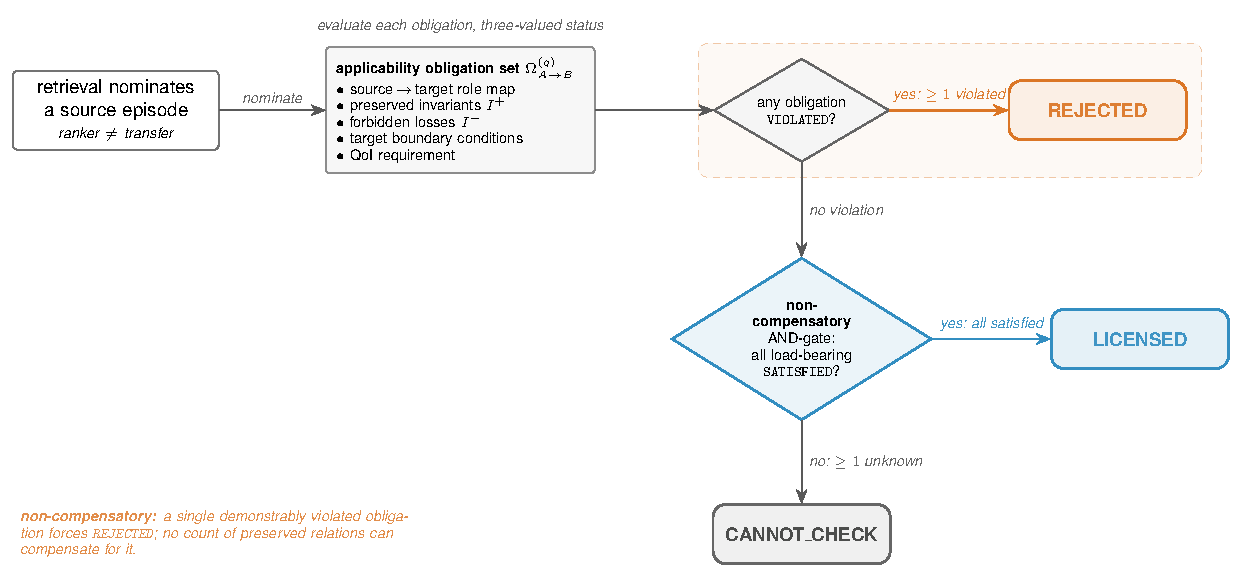
\includegraphics[width=\textwidth]{figures/transfer_decision.pdf}
\caption{The fail-closed transfer decision. A nominated source is evaluated against the applicability obligation set (role map, preserved invariants $I^+$, forbidden losses $I^-$, target boundary, QoI), each with a three-valued status. The rule is non-compensatory: any single demonstrably violated load-bearing obligation forces \texttt{REJECTED}; only when every load-bearing obligation is satisfied is the transfer \texttt{LICENSED}; an unresolved obligation yields \texttt{CANNOT\_CHECK}. No count of preserved relations can buy back a violation.}
\label{fig:transfer-decision}
\end{figure}

\subsection{Why explicit non-preservation matters}

Analogies are dangerous when the reusable part and the non-reusable part are stored in one undifferentiated similarity score. The witness therefore records $I^-$. In the queue example, ``arrival competes with service and excess load grows backlog'' may transfer while domain-specific priority policy and entity semantics do not. This is more than documentation: a later operator can declare which preserved invariants it depends on, and an intervention touching a non-preserved property can fail closed. We found no counterpart to this explicit forbidden-loss enumeration in any of the literature families searched in Section~\ref{sec:parents}; it is one of the four surviving residuals.

\subsection{Where the contract sits in the deployed router}

Orion's obstruction--transformation router gives the witness a precise operational location. The router fingerprints the active target obstruction using roles, relations, constraints, failure mechanisms, invariants to preserve, desired transition and forbidden losses, then queries a content-bound memory of recorded source episodes $O_s\xrightarrow{T_s}O_s'$. A semantic or structural ranker may nominate a source, but source retrieval is not yet transfer. For a cross-domain \texttt{JUMP}, the source transformation becomes a viable target proposal only when a mapping witness accounts for the load-bearing source structure: source-to-target role mapping, shared relations and constraints, every enabling source precondition, material disanalogies and target-domain validation obligations. An unrepaired source precondition or a conflict with a forbidden target invariant blocks the transfer even when the source event itself is well verified. For \texttt{GLUE}, partial episodes whose combined recorded effects cover the desired transition remain composition candidates only; a separate composition witness must bind operation order, interfaces and incompatibility checks. Directional witnesses license transport of components; they do not prove that a composed pipeline is coherent.

This yields the three-stage distinction of Figure~\ref{fig:transfer-ladder}:
\[
\text{retrieved source}
\;\neq\;
\text{witnessed target applicability}
\;\neq\;
\text{verified target success}.
\]
This paper studies the middle relation. When a witness passes, Orion may raise retrieval priority, activate an already promoted tool, or place an operator path earlier in the search queue. The permitted inference is witnessed applicability $\Rightarrow$ eligible experience reuse, \emph{not} witnessed applicability $\Rightarrow$ scientific claim true. Scientific authority remains owned by the target problem's verification path---the cross-domain specialization of the companion paper's invariant that experience-conditioned routing is not epistemic authority \cite{yiu2026epistemic}.

\begin{figure}[t]
\centering
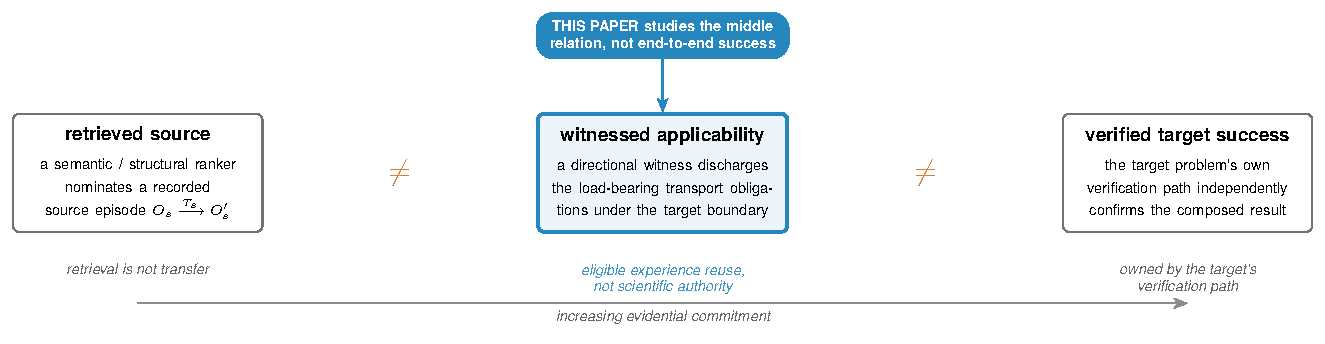
\includegraphics[width=\textwidth]{figures/transfer_ladder.pdf}
\caption{Three stages of increasing evidential commitment. A retriever nominating a source episode is not the same as a directional witness discharging the load-bearing transport obligations under the target boundary, which is in turn not the same as the target problem's own verification path independently confirming success. This paper's subject is the middle relation---witnessed applicability---which licenses eligible reuse without minting scientific authority; retrieval and end-to-end success are owned by other stages.}
\label{fig:transfer-ladder}
\end{figure}

\subsection{Negative transfer is recorded through an evidence ladder}

A failed transfer attempt first creates a non-success task episode. It does not immediately establish that the witness class, operator or source lesson is invalid. The system records the failure as observed-only, then permits competing diagnoses such as context mismatch, broken invariant, implementation defect, missing evidence or an unrelated downstream failure. Only discriminating evidence can promote a supported diagnosis, and only fresh replay/transfer can turn that diagnosis into a reusable boundary lesson. This prevents one near-miss from becoming a global blacklist while still allowing repeated boundary-sensitive failures to improve later routing, and it makes negative-transfer history addressable: a future witness can explicitly inherit a known non-preserved property or target boundary rather than merely receiving a lower opaque score.

\subsection{Exact scope of the specification claim}

The claim of this section is that the contract is (i) executable---the reference implementation evaluates obligation sets deterministically and emits content-hashed traces; (ii) fail-closed---missing evidence yields abstention, not a score; and (iii) exactly scoped---each verdict names the QoI, boundary and obligation set it is conditional on. The claim is \emph{not} that the contract improves transfer decisions on any natural distribution of problems, that its coordinates can be recovered from natural prose, or that its verdicts correlate with downstream research utility. Those are empirical questions; their current evidential status---including the refutation of two of our own instruments and the template-inversion terminal of a third---is reported in Sections~\ref{sec:falsifiability}--\ref{sec:natural-domain}.
